
%%%%%%%%%%%%%

\documentclass[10pt,a4paper,titlepage]{paper}
\setcounter{secnumdepth}{5}
\usepackage[a4paper, left=2cm, right=2cm, top=1.6cm, bottom=2.5cm]{geometry}
\usepackage[utf8]{inputenc}
\makeatletter
%%%%%%%%%%%%%%%%%%%%%%%%%%%%%%% sub sub sub section :) mit paragraph{text}
\renewcommand\paragraph{\@startsection{paragraph}{4}{\z@}%
            {-2.5ex\@plus -1ex \@minus -.25ex}%
            {1.25ex \@plus .25ex}%
            {\normalfont\normalsize\bfseries}}
\makeatother
\setcounter{secnumdepth}{4} % how many sectioning levels to assign numbers to
\setcounter{tocdepth}{4}    % how many sectioning levels to show in ToC
%%%%%%%%%%%%%%%%%%%%%%%%%%%%%%%%%%%%%%%%%%%%%%%%%%%%%%
\usepackage{pst-all}
\usepackage{pst-circ}
\usepackage{amsmath}
\usepackage[ngerman]{babel}
\usepackage{amsfonts}
\usepackage{amssymb}
\usepackage{caption}
\usepackage{color}
\usepackage{framed}
\usepackage{ntheorem}
\usepackage{epsfig}
%\usepackage[pdftex]{graphicx}
\usepackage{pstricks}
\usepackage{placeins}
\usepackage{caption}
\usepackage{tabularx}
\usepackage{hyperref}
\usepackage{fancyhdr}
\usepackage{fancyvrb,newverbs,xcolor}
\usepackage{lipsum}% just for this example
\usepackage{pdfpages}
\usepackage{fourier} 
\usepackage{array}
\usepackage{makecell}
%für echte hochkommas statt einfachen anführungszeichen
\usepackage{upquote}
\renewcommand\theadalign{bc}
\renewcommand\theadfont{\bfseries}
\renewcommand\theadgape{\Gape[4pt]}
\renewcommand\cellgape{\Gape[4pt]}

\definecolor{cverbbg}{rgb}{0.9, 0.95, 1.0}


\newenvironment{cverbatim}
 {\SaveVerbatim{cverb}}
 {\endSaveVerbatim
  \flushleft\fboxrule=0pt\fboxsep=.5em
  \colorbox{cverbbg}{\BUseVerbatim{cverb}}%
  \endflushleft
}

\definecolor{pverbbg}{rgb}{0.97, 0.91, 0.81}

\newenvironment{pverbatim}
 {\SaveVerbatim{cverb}}
 {\endSaveVerbatim
  \flushleft\fboxrule=0pt\fboxsep=.5em
  \colorbox{pverbbg}{\BUseVerbatim{cverb}}%
  \endflushleft
}

\pagestyle{fancy}
\lhead{Cyber-security - Passwords: Version 0.1}
\rhead{Team HTL Anichstraße (February 2023)}

% Befehl für farbige Rahmen
\definecolor{rotlich}{rgb}{1,.9,.9}
\definecolor{gruenlich}{rgb}{.9,1,.9}
\definecolor{blaulich}{rgb}{.9,.9,1}

\begin{document}

\pagenumbering{roman}
%\pagestyle{plain}
\begin{center}
		\vspace*{1cm}
		
		\Huge \bf Passwords\\
		\vspace{5cm}
		
		%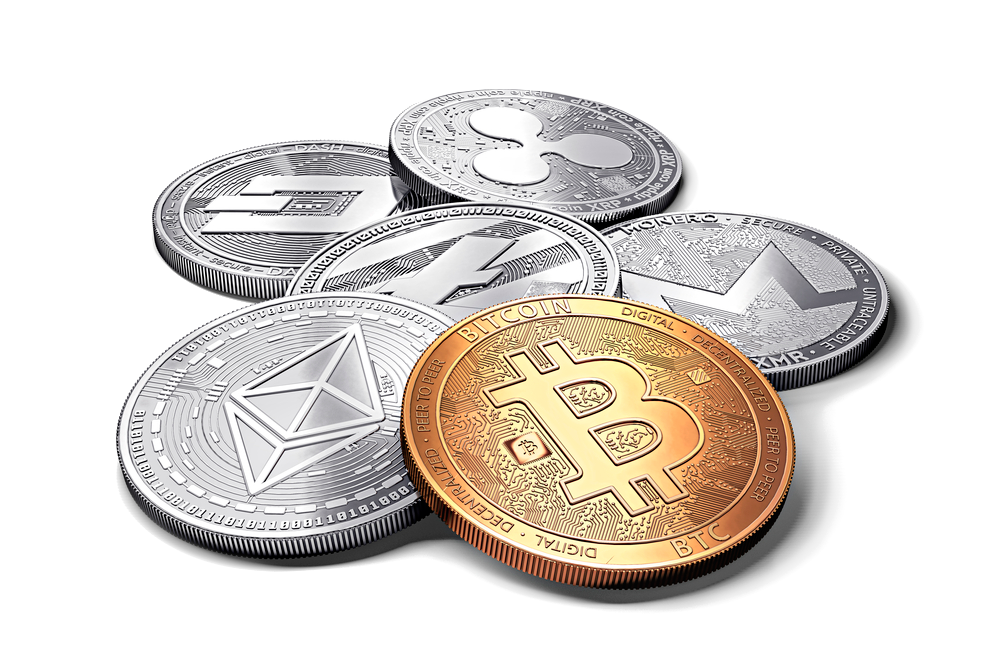
\includegraphics[scale=.35]{./images/title.png}\\
		
		
		
		
		\vspace{1.5cm}
		\huge A brief summary of solutions to the never dying problems of pins. \\
		\vspace{2cm}
		\Large Basierend auf dem Buch \textit{Bitcoin ohne Vorkenntnisse} von Benjamin Spahic,\\ sowie diversen Online-Artikeln.
		\vspace*{1.5cm}
		
		\Large Version 0.1\\
		\large Febuary 2023\\
		\large Team HTL Anichstraße\\[30pt]
		\vspace{1cm}
		
		
		\vspace*{5cm}	
	
		

        \large no \copyright\ by Lilo Zobl\\
        
\end{center}
\newpage    %Ende der Titelseite


% Inhaltsverzeichnis
\addtocontents{toc}{\protect\thispagestyle{empty}} 
\tableofcontents
\newpage
%Abbildungsverzeichnis erstellen
\listoffigures
\listoftables
\clearpage
% ab sofort wieder mit arabischen Seitenzahlen
\pagenumbering{arabic}

\section{Abstract}


\section{Introduction}
Password. Everyone has one or rather multiple. But it's a faulty construction. Nowadays passwords are everything but a good invention.\\ These are the reasons: i) Passwords are not user-friendly. In order to make passwords securer providers make them complexer. User have to write them down or use the same one over and over so they don't forget it. ii) Passwords are not secure because they can be shared and guessed. Of course a lot of passwords are also stolen, which is a lot easier than anyone would think. iii) Passwords are weak and get reused. Here are some examples to the most frequently used ones of 2022: "password", "123456", "123456789", "guest", "qwerty", ect.\\
Luckily there is a websites that lets users check if their account information was breached (that's when your email connected to a password is leaked; always a huge amount of accounts get breached from a branch such as Facebook). The website is called "haveibeenpwned.com". HIBP is open source and secure. If someone searches for a breach it doesn't store the data that was typed in (an email address or phone number). It only ever retrieves the data from storage then returns it in the response. 
%ich würd gern ein bild von der Seite einfügen hier

\section{Haupteil?}
Passwords have always been a security threat ever since they where introduced. Providers have tried to find solutions such as requiring users to make the pin at least eight characters long or use upper case and lower case letters. Sometimes they require you to include digits or symbols. However those "solutions" didn't improve the situation overall and sometimes made it worse.
To eliminate this security threat a few solutions created.

\subsection{Password Save}
\subsubsection{Explanation}
A password save allows you to save a list of your usenames linked to the password. It has one master password that looks the save. Instead of remembering a ton of password at once users only have to recall one single pin. The rest is done by the app or rather the software.
\subsubsection{Providers}
\begin{itemize}
\item \textbf{KeepassXC}\\
This software is developed for users with extremely high demands of secure personal data management. \\
KeePassXC uses Advanced Encryption Standard (AES) encryption algorithm with a 256-bit key to secure the password database.\\
The biggest difference to other password saves is that the data (password, account information and additional data such as URLs, attachments ans notes) is stored in an offline, encrypted file that can be stored locally. This prevents your data from getting leaked when the could gets hacked or breached.\\
The program is customizable. It allows its user to customize literally everything to their needs.\\

\item \textbf{1Passwort}\\
This password save is known for its easy to use interface and high security encryption.\\
1Password uses an uncommon encryption known as dual-key encryption. If the server gets breached it's impossible for the hacker to decrypt the users sensitive information because of its two keys. The first key is the users master-key. The second key is a secret key, which is a 128-bit, machine-generated code. The secret key is generated on every device you log into. It will only be saved on your devices and never saved with your other pins.\\
Depending on what account type you choose your data is stored differently. However in only one version users have the option to save their data locally. In every other option the user's data gets saved in a cloud-based vault.\\
The interface is very user-friendly. It even creates strong passwords for accounts that are newly created.
\item \textbf{Password Safe (MATESO)}\\

\item \textbf{LastPass}\\
\item \textbf{Dashlane}\\
\end{itemize}


\subsection{2-factor authentication}
\subsection{The future of passwords}

\section{conclusion}

\section{Grundlagen der Kryptographie}
Durch bekannte, erprobte Verschlüsselungsalgorithmen werden Transaktionen
verschlüsselt, durchgeführt und bestätigt.
\begin{center}
\textit{„Die Verschlüsselung funktioniert. Richtig implementierte starke
Kryptosysteme sind eines der wenigen Dinge, auf die wir uns verlassen können“. - Edward Snowden}
\end{center}
\subsection{Die drei Ziele der Kryptographie}
\begin{itemize}
\item \textbf{Integrity (Datenintegrität)\\ Wie können wir sicher sein, dass Daten unverfälscht sind?}\\ Mit sogenannten Hashing-Funktionen (für mehr Details siehe Kapitel \ref{hash} auf Seite \pageref{hash})\\ Aktueller Standard: Secure Hash Algorithm 2 (SHA2); Beispiel: Wird auch oft bei Downloads angeboten um zu überprüfen, ob das heruntergeladene File mit dem am Server übereinstimmt. 
\item \textbf{Authentication (Authentifizierung)\\ Wie können wir sicher sein, dass die Daten auch tatsächlich vom vermutlichen Absender stammen?}\\Mit keyed Hashes (siehe Kapitel \ref{hmac} auf Seite \pageref{hmac}) oder asymmetrischer Verschlüsselung (siehe Kapitel \ref{asym} auf Seite \pageref{asym}). Beispiel Algorithmen: HMAC-MD5, HMAC-SHA-1, RSA und DSA;
\item \textbf{Confidentiality (Vertraulichkeit)\\ Wie können wir sicher sein, dass die Daten von niemand anderem gelesen werden können?}\\Mit klassischer Verschlüsselung (symmetrisch oder asymmetrisch). Beispiel Algorithmen: DES, 3DES, AES, SEAL, Elliptic-Curve;
\end{itemize}

\newpage
\subsection{Datenintegrität - Hashing} \label{hash}
\textbf{Hashes} werden verwendet um die \textbf{Integrität} einer Nachricht oder eines Files sicherzustellen. Hashing basiert auf einer \textbf{mathematischen Einweg-Funktion} - einfach durchzuführen aber schwer umzudrehen, wie zum Beispiel das Kaffee mahlen: Es ist einfach aus Kaffeebohnen Kaffeepulver zu mahlen, aber aus dem Pulver wieder die Bohnen zusammensetzen ist eher schwierig ;-)\\
\begin{minipage}{6.7cm}
\textbf{Prinzip}:\\Aus einer beliebig langen Nachricht oder einem File-Inhalt wird durch hashing ein Hash-Value mit einer fixen Länge erzeugt.
Beim Hashing wird der ursprüngliche Inhalt in mehreren Stufen verschoben, vertauscht, komprimiert oder ergänzt. Wie genau ist immer vom verwendeten Hashing-Algorithmus abhängig.\\
Am Ende dieser Prozedur entsteht ein immer gleich langer (bei SHA256 z.B: 256 bit) Hash-Wert.\\ Jede noch so kleine Änderung in der Nachricht oder dem File erzeugt ein unterschiedliches Hash-Value. Hashes werden deshalb auch oft als digitale Fingerabdrücke bezeichnet. 
\end{minipage}
\begin{minipage}{8cm}
\begin{center}

%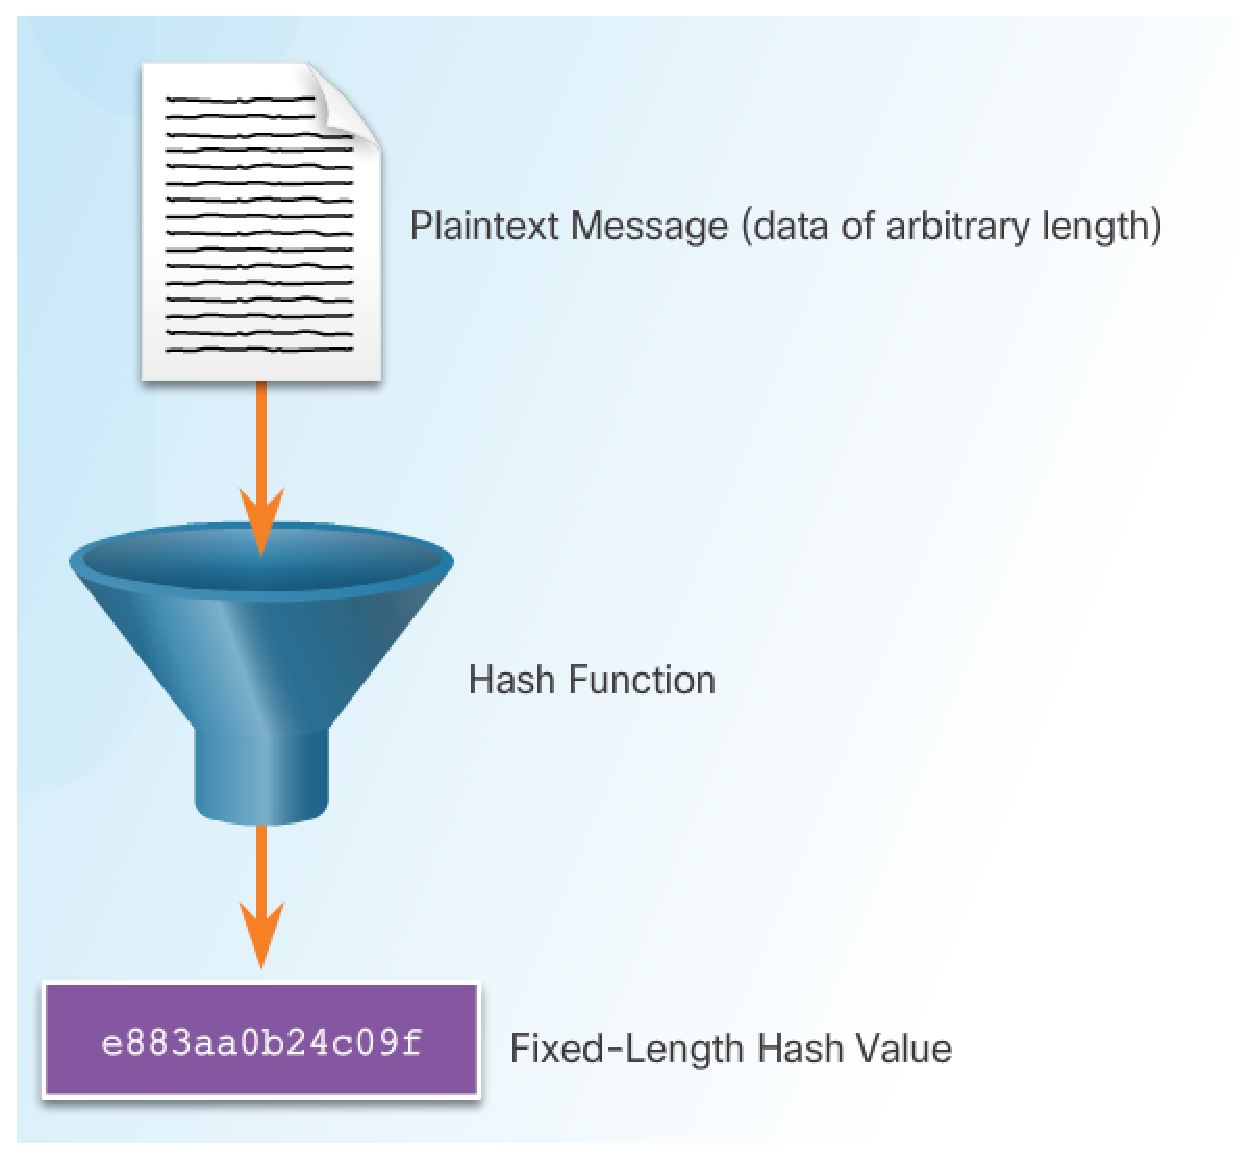
\includegraphics[scale=0.35]{./images/hash.eps}
\captionof{figure}[Hashing Function - die Abbildung stammt vom Cisco Netacad Network Security Kurs]{Hashing Function}

\end{center}
\end{minipage}
\subsection{SHA}
Hashing Algorithmen werden laufend weiterentwickelt. Der aktuell am weitesten verbreitete Algorithmus ist \textbf{SHA}.\\ \textbf{SHA steht für  Secure Hash Algorithm}, und wurde vom National Institute of Standards and Technology (NIST) entwickelt; Erste Version stammt von 1994, aktuelle Versionen wurden im August 2002 (SHA-2-Familie) vorgestellt und sind SHA-256, SHA-384, SHA-512. Die nächste Generation (SHA-3-Familie) wurde 2015 vorgestellt.\vspace{.3cm}\\
\textbf{SHA-256} hat auch für die Funktionsweise von Bitcoin eine große Bedeutung. Mehr dazu sie Kapitel \ref{mining} auf Seite \pageref{mining}.
\vspace{.5cm}\\
File-Hash berechnen unter Linux - Darstellung in hexadezimaler Schreibweise!
\begin{cverbatim}
sha256sum ./main.jpg 
a7f837e28843fba098c0929037743d28edf6a97ed74ff17127aa329423acf52c  ./main.jpg
\end{cverbatim}
File-Hash berechnen unter Windows in der Power-Shell
\begin{cverbatim}
Get-FileHash C:\Users\user1\Downloads\file.txt -Algorithm SHA256 | Format-List

Algorithm : SHA256
Hash      : 3CBCFDDEC145E3382D592266BE193E5BE53443138EE6AB6CA09FF20DF609E268
Path      : C:\Users\user1\Downloads\file.txt
\end{cverbatim}
Für mehr Informationen zur genauen Funktionsweise von SHA-256 siehe:\\
\href{https://en.wikipedia.org/wiki/SHA-2}{\color{blue}https://en.wikipedia.org/wiki/SHA-2}

\newpage
\subsection{HMAC} \label{hmac}
Hash Message Authentication Code (HMAC) oder auch manchmal Keyed-hash message authentication code (KHMAC) sind Hashes die noch einen zusätzlichen, geheimen Schlüssel verwenden. 
\begin{center}
%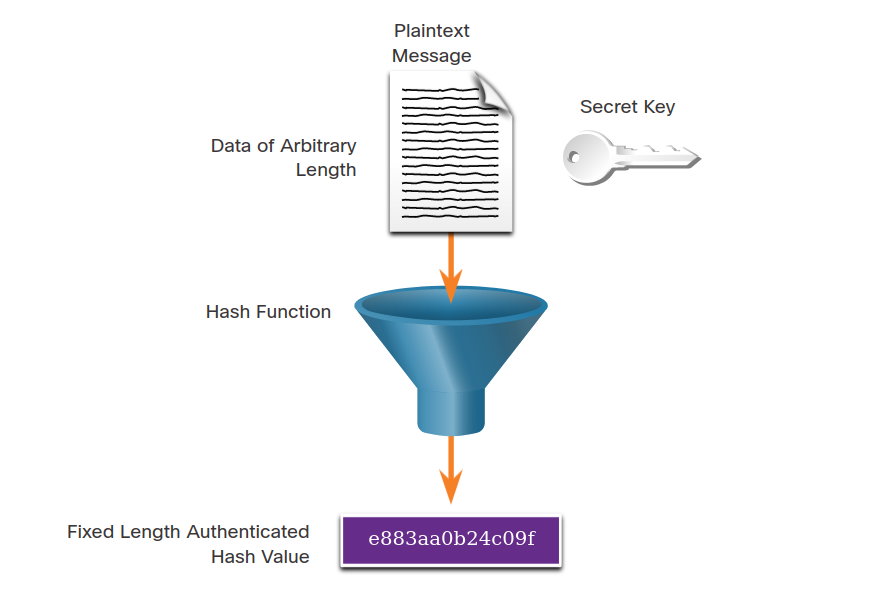
\includegraphics[scale=0.4]{./images/hmac.png}
\captionof{figure}[HMAC - die Abbildung stammt vom Cisco Netacad Network Security Kurs]{HMAC - hash bases message authentication}
\end{center}
Nur wer die Daten und den geheimen Schlüssel hat kann den richtigen Hash-Wert berechnen.

\subsection{Verschlüsselung - Vertraulichkeit}
Es gibt verschiedene Verschlüsselungsmethoden. Prinzipiell lässt sich eine Einteilung in symmetrische und asymmetrische Verfahren treffen.

\subsubsection{Symmetrische Verschlüsselung}
Symmetrisch bedeutet, dass sowohl für die Verschlüsselung als auch für die Entschlüsselung \textbf{der gleiche Schlüssel} verwendet wird.\\
\begin{center}
%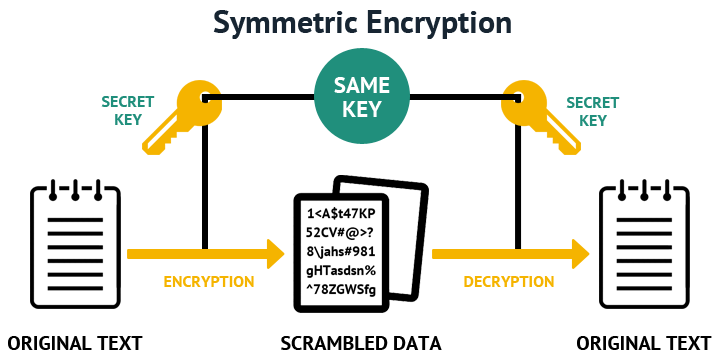
\includegraphics[scale=0.43]{./images/symmetric-encryption.png}
\captionof{figure}[Symmetric-Encryption - die Abbildung stammt vom https://www.cheapsslshop.com/blog/symmetric-vs-asymmetric-encryption-whats-the-difference]{Symmetrische Verschlüsselung}
\end{center}
Symmetrische Verfahren sind meist \textbf{schnell} (schneller als asymmetrische Verfahren) und verwenden im Vergleich zu asymmetrischen Verfahren eher kurz Schlüssel.\\
Die eigentliche Übersetzung kann blockweise erfolgen (z.B. es werden jeweils 128 Bit der Nachricht übersetzt) - dann spricht man von einem \textbf{Block Cipher}, oder Bit by Bit - dann spricht man von \textbf{Stream Chiper}.\vspace{.3cm}\\
\textbf{AES} (Advanced Encryption Standard) ist zur Zeit (seit dem Jahr 2000) der etablierte Standard für symmetrische Verschlüsselung. Es ist ein Blockcipher mit 128 Bit Länge und die Schlüssellänge kann 128, 192 oder 256 Bit betragen.\\
Für mehr Info zu AES siehe:\\
\href{https://de.wikipedia.org/wiki/Advanced_Encryption_Standard}{\color{blue}https://de.wikipedia.org/wiki/Advanced\_Encryption\_Standard}\vspace{.3cm}\\
Das eigentliche \textbf{Problem} bei symmetrischen Verfahren liegt im \textbf{Schlüsselaustausch}! Wie schafft man es über ein unsicheres Medium einen geheimen Schlüssel auszutauschen?\\
Aber auch dafür gibt es Lösungen, z.B. den Diffie-Hellmann Key Exchange, aber dies sprengt den Rahmen dieses Skripts. Mehr dazu gibt es im Fach Netzwerktechnik!
\subsubsection{Asymmetrische Verschlüsselung} \label{asym}
Wird auch \textbf{Public Key Encryption} genannt.\\
Die asymmetrische Verschlüsselung umgeht das Problem des Key-Exchanges in dem es pro Teilnehmer \textbf{zwei Schlüssel} gibt: einen Public Key und einen Private Key. Die Besonderheit an den Keys ist, dass eine Message, die mit einem der Keys verschlüsselt wurde, nur mit dem anderen Key entschlüsselt werden kann! Der öffentliche Schlüssel und der private Schlüssel hängen über mathematische Funktionen zusammen. Es ist jedoch nicht möglich, von dem öffentlichen Schlüssel auf den privaten Schlüssel zurück zu schließen.
\begin{center}
%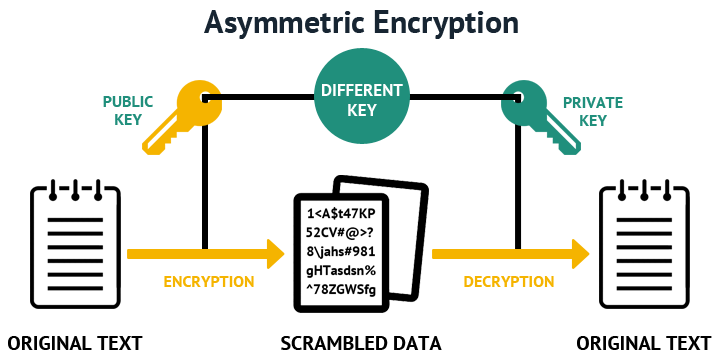
\includegraphics[scale=0.43]{./images/asymmetric-encryption.png}
\captionof{figure}[Asymmetric-Encryption - die Abbildung stammt vom https://www.cheapsslshop.com/blog/symmetric-vs-asymmetric-encryption-whats-the-difference]{Asymmetrische Verschlüsselung}
\end{center}
Es gibt mehrere asymmetrische Verschlüsselungsverfahren z.B. RSA oder ECC. Sie sind in der Regel deutlich langsamer als symmetrische Verfahren, umgehen aber das Problem des Schlüsselaustauschs und erlauben zusätzlich zur Confidentiality auch noch Integrity und Authentication!
\begin{itemize}
\item \textbf{Public Key (Encrypt) + Private Key (Decrypt) = Confidentiality}\\Schickst Du mir etwas mit meinem Public Key, kann nur ich es mit meinem Private Key lesen!
\item \textbf{Private Key (Encrypt) + Public Key (Decrypt) = Authentication}\\Schicke ich dir etwas mit meinem Private Key, kann es nur von mir gekommen sein, weil nur ich den Private Key habe - lesen kann es jeder, der meinen Public Key hat. Dies nennt man auch eine \textbf{signierte} Nachricht oder \textbf{digitale Signatur}!
\item \textbf{Confidentiality, Authentication und Integrity?} - geht auch:\\
Ich schicke dir eine Nachricht mit deinem Public Key, aber zusätzlich bilde ich noch einen Hash der Nachricht mit meinem Private Key! Du entschlüsselst die Nachricht mit deinem Private Key und überprüfst den Hash mit meinem Public Key - damit ist sicher gestellt, dass die Nachricht von mir ist und nicht verändert wurde (wenn der Hash übereinstimmt).
\end{itemize}

\paragraph{ECC - Eliptic Curve Cryptography} \label{ECC}
Bitcoin verwendet ECC um aus einem Private Key (256 Bit Länge - meist als Zufallszahl erzeugt) einen Public Key zu erzeugen.\\
Achtung: Es gibt eine technische Einschränkung: Der Private Key muss zwischen \verb|0| und \verb|n-1| liegen wobei \verb|n=1,1578*10^77| ist und mit der elliptischen Kurve zu tun hat (Order der Kurve) die Bitcoin verwendet.\\
Der Public Key wird durch \textbf{Elliptische Kurvenmultiplikation} mit der Formel $K=k*G$ erzeugt. Wobei $k$ der Private Key ist. $G$ der \textit{generator point} - ein Punkt auf der elliptischen Kurve und $K$ der resultierende Public Key. Achtung: Der Operator $*$ ist keine normale Multiplikation, sondern eine elliptische Kurvenmultiplikation!\\
Die Besonderheit dabei ist, das $K$ aus $k$ und $G$ relativ einfach berechnet werden kann, aber die Umkehrfunktion, nämlich $k$ aus $K$ und $G$ zu berechnen, nahezu unmöglich ist.\\
Bitcoin verwendet eine elliptische Kurve aus dem \verb|secp256k1| Standard, der vom amerikanischen NIST (National Institute of Standards and Technology) vorgestellt wurde.\\
\subparagraph{Elliptische Kurven Multiplikation}
Im folgenden wird eine vereinfachte Kurve verwendet, um das Prinzip der elliptischen Kurven Multiplikation zu erklären - sie entspricht nicht der von Bitcoin verwendeten Kurve!\\
\textbf{ECC-Multiplikation} bedeutet, dass man die Tangente (differenzieren - erste Ableitung) zum Ausgangspunkt $G$ nimmt und schaut, wo sich diese mit der Kurve kreuzt ($-2G$). Dann springt man auf die andere Seite der Kurve und erhält $2G$. Weitere Multiplikation ergibt $4G$, $8G$ usw.
\begin{center}
%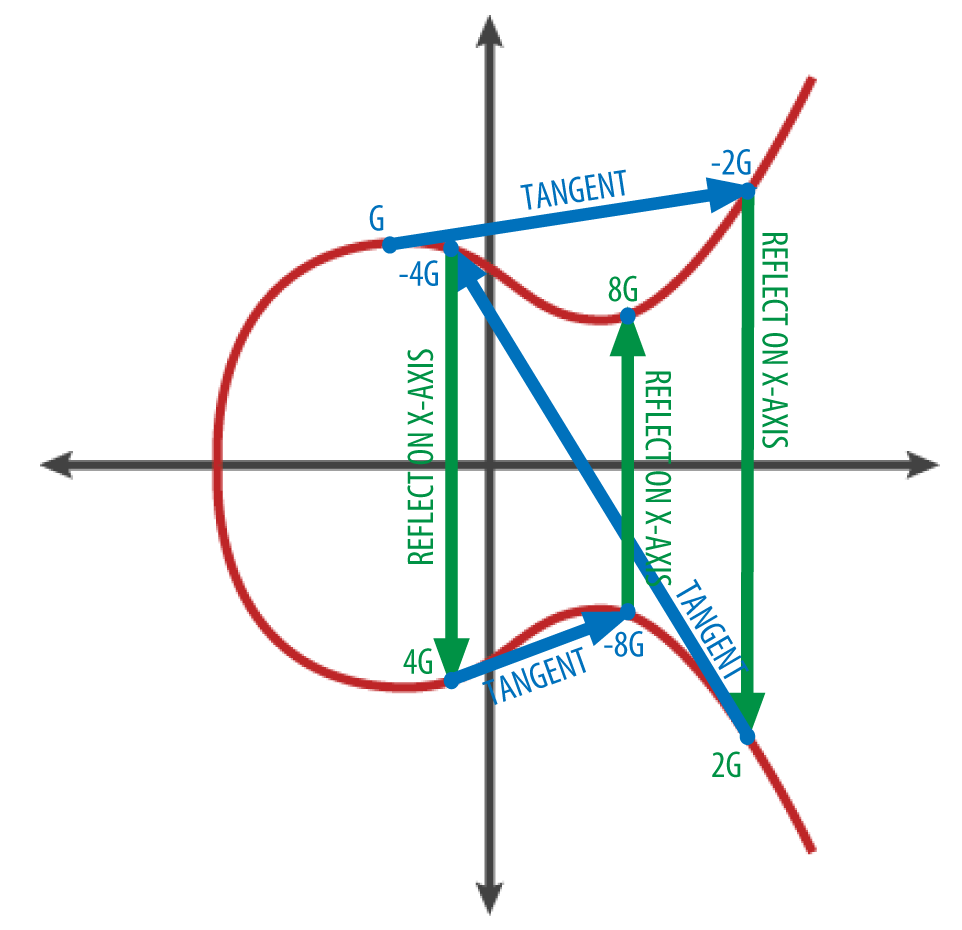
\includegraphics[scale=0.3]{./images/curve.png}
\captionof{figure}[ECC-Multiplication - die Abbildung stammt vom https://www.oreilly.com/library/view/mastering-bitcoin-2nd/9781491954379/ch04.html]{ECC-Multiplikation veranschaulicht}
\end{center}
Der Private Key gibt also an, wie oft ECC-Multiplikationen durchgeführt werden müssen, um den Public Key zu erhalten.
z.B.: Private Key = 2 führt zu Public Key = 4G, Private Key = 3 führt zu Public Key 8G, usw.
%\newpage
\section{Die Entstehung von Bitcoin}
Nach der Finanzkrise 2008 hat eine Person oder ein Kollektiv, unter dem Pseudonym \textbf{Satoshi Nakamoto}, eine digitale, dezentrale und begrenzte Währung erschaffen: den Bitcoin. Es ist bis heute ungeklärt, wer Satoshi Nakamoto wirklich ist.\vspace{.3cm}\\
Link zum ursprünglichen White-Paper:\\
\href{https://bitcoin.org/bitcoin.pdf}{\color{blue}https://bitcoin.org/bitcoin.pdf}\vspace{.3cm}\\
Link zum Bitcoin-Sourcecode auf Github:\\
\href{https://github.com/bitcoin/}{\color{blue}https://github.com/bitcoin/} \vspace{.3cm}\\
Die Grundlage der Digitalen Währung sind:
\begin{itemize}
\item \textbf{Transparenz}\\alle Transaktionen werden in einer Blockchain aufgezeichnet und sind seit der ersten Transaktion einsehbar.
\item \textbf{Sicherheit}\\die Blockchain ist im Nachhinein nicht mehr (nur sehr schwer) änderbar.
\item \textbf{Dezentralisierung}\\die Kopien der Blockchain liegen verteilt im Netz (Full-Nodes) und werden regelmäßig aktualisiert.
\item \textbf{Inflationssicherheit}\\es gibt nur eine begrenzte Anzahl an Bitcoins (21 Millionen)  
\end{itemize} 

\subsection{Bitcoin, mBTC und Satoshi - die Währungseinheiten}
Ähnlich wie es beim Euro noch Euro-Cents gibt, gibt es auch bei Bitcoin (\textbf{BTC}) kleinere Einheiten: Den Milli-Bitcoin (\textbf{mBTC}) und den \textbf{Satoshii}. Es gilt:
\begin{center}
\verb|1 BTC = 1000 mBTC = 100.000.000 Satoshii|
\end{center} 

%\newpage
\section{Blockchain}
Im folgenden wird der Aufbau einer Blockchain am Beispiel von Bitcoin erklärt, das Prinzip kann aber auf beliebige Daten (nicht nur Bitcon-Transaktionen) angewandt werden.
\subsection{Aufbau der Blockchain}
Die Blockchain besteht aus Blöcken. Der \textbf{erste Eintrag} eines Blocks ist immer ein \textbf{Verweis} auf den \textbf{vorherigen Block}. Dadurch ist die Verbindung zum vorherigen Block festgelegt und die Blöcke verknüpfen sich zu einer Kette.\\
Bei Bitcoin enthält ein Block eine Reihe von Transaktionen die in einem bestimmten Zeitraum angefallen sind.\\
Die Blockgröße ist bei Bitcoin ursprünglich auf 1 MByte limitiert (ist inzwischen auf 4MByte angehoben, aber die durchschnittliche Blockgröße ist bei ca. 1,13 MByte). Dadurch können pro Block ca. 2000 Transaktionen durchgeführt werden.
Über die gesamten Daten eines Blocks wird mittels SHA-256 ein Hash gebildet.
\begin{center}
%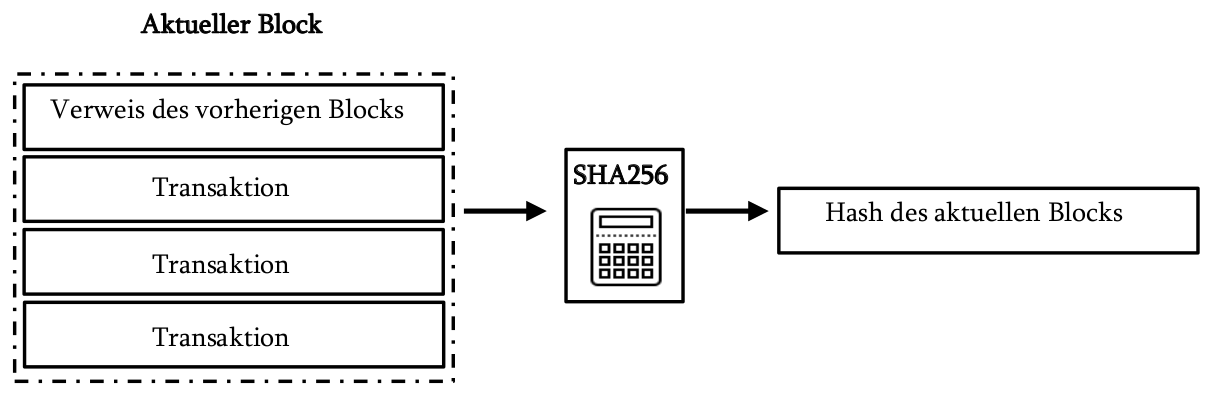
\includegraphics[scale=0.4]{./images/block.png}
\captionof{figure}[Abbildung 22 aus dem Buch: Bitcoin ohne Vorkenntnisse]{Hash-Generierung aus den Daten eines Blocks}
\end{center}
Ändern wir nur ein Zeichen des gesamten Blocks, ändert sich der Hash
vollständig und unvorhersehbar. Eine einzige Änderung in nur einer Transaktion würde den kompletten Hash des Blocks und damit alle weiteren Blöcke verändern.\\
Somit ist der Hash des aktuellen Blocks gleichzeitig ein eindeutiger Verweis auf diesen Block. Der Hash des aktuellen Blocks wird als erster Eintrag des Folgeblocks eingesetzt. So entsteht eine Reihenfolge von Blöcken - die Blockchain.
\begin{center}
%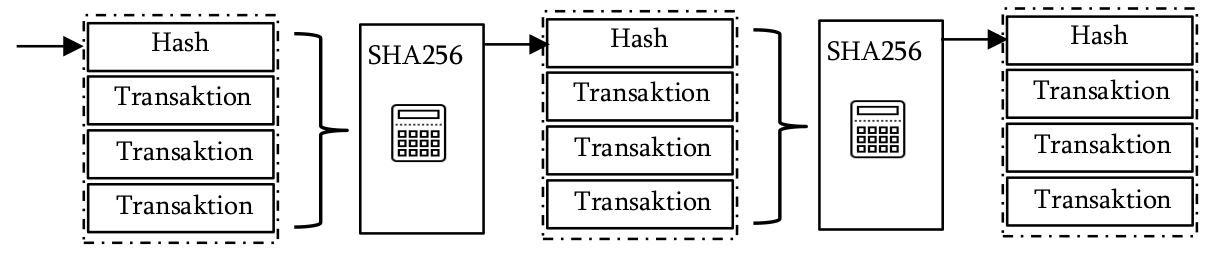
\includegraphics[scale=0.4]{./images/blocks.png}
\captionof{figure}[Abbildung 23 aus dem Buch: Bitcoin ohne Vorkenntnisse]{Aneinanderreihung von Blöcken}
\end{center}
Der erste Block in der Blockchain ist vorgegeben und wird \textbf{Genesisblock} genannt. 
\subsection{Dezentralisierung, Full-Nodes und Größe}
\textbf{Dezentralität} bedeutet, dass es keine zentrale Institution wie  z.B. eine Bank oder einen Staat gibt, der über ein System (die Blockchain) wacht. Stattdessen liegen viele Kopien der Blockchain verteilt in einem großen Netzwerk. Jeder Teilnehmer des Netzwerks, welcher die \textbf{volle Transaktionshistorie} (also die gesamte Blockchain) hostet, wird \textbf{Full-Node} genannt.\\
Damit jeder Knotenpunkt des Netzwerks (Full-Nodes) die aktuelle Blockchain besitzt, wird die Blockchain in regelmäßigen Abschnitten aktualisiert und an jeden Teilnehmer übermittelt.
Nach einem gewissen zeitlichen Abschnitt, bei Bitcoin alle zehn Minuten, wird ein Paket mit neuen Informationen, ein sogenannter Block, an die bisherige Transaktionshistorie angehängt. Das hat den Vorteil, dass nicht jede einzelne Transaktion aktualisiert werden muss, sondern ein Bündel von Transaktionen.\\
Die zehn Minuten werden durch den Bitcoin Algorithmus gesteuert, indem die Mining-Difficulty angepasst wird. Mehr dazu siehe im Kaptiel \ref{mining} auf Seite \pageref{mining}.
Die \textbf{momentane Größe} (Oktober 2022) der Bitcoin-Blockchain liegt bei ca. 432 GByte. Zum Startzeitpunkt von Bitcoin (03.01.09) war sie 285 Byte groß. 
\begin{center}
%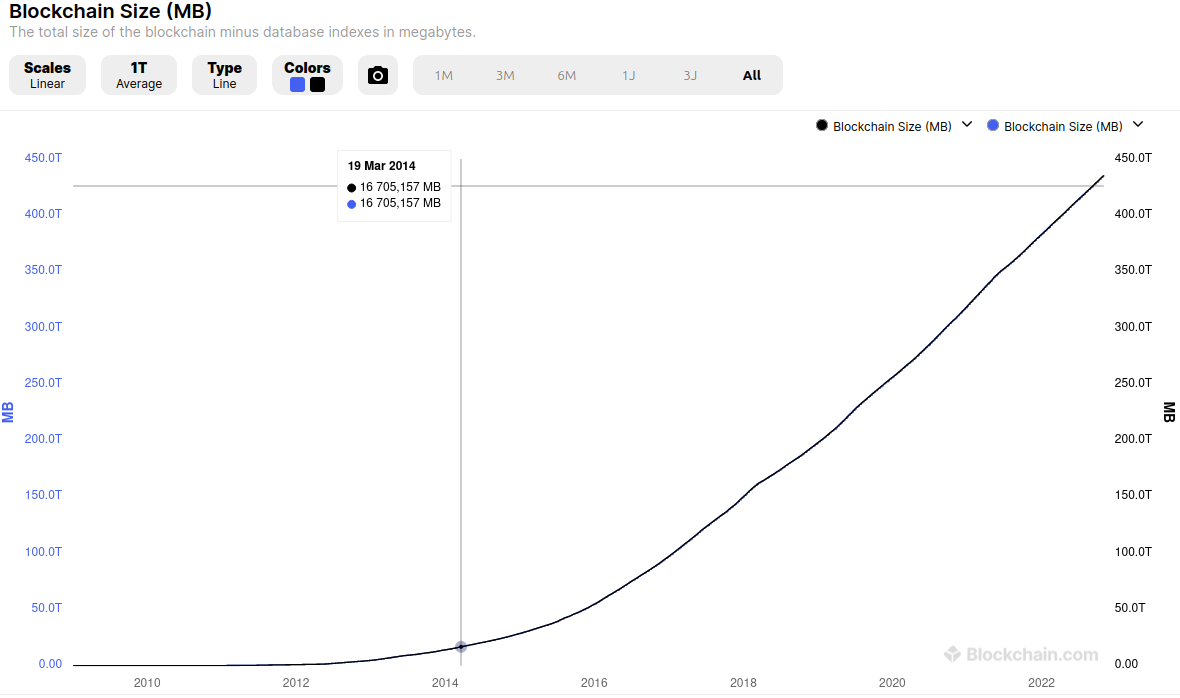
\includegraphics[scale=0.35]{./images/bc-size.png}
\captionof{figure}[https://www.blockchain.com/explorer/charts/blocks-size]{Wachstum der Bitcoin Blockchain seit 2009}
\end{center}

\subsection{Konsensbildung in einem dezentralisiertem System}
Wenn jeder Full-Node eine Kopie der Blockchain hat, und sie theoretisch verändern kann, wer hat dann die \textit{richtige} Blockchain?\\
Gültige Blöcke werden nur durch das rechenintensive \textbf{Mining} (siehe Kapitel \ref{mining} auf Seite \pageref{mining}) erschaffen. So vertraut jeder Bitcoin-Node der \textbf{längsten gültigen Blockchain}, da hinter dieser die meiste Rechenleistung steht und deswegen auch die Mehrheit der Teilnehmer vermutet wird. Man kann also vereinfacht sagen: \textit{Die Mehrheit bestimmt was wahr ist.} \\
Dies kann unter bestimmten Umständen problematisch werden - siehe \textit{51\% Angriff} im Kapitel \ref{51} auf Seite \pageref{51}.\\
\subsubsection{Konsensmechanismen}
Es gibt mehrere Konsensverfahren. Die zwei bekanntesten sind:
\paragraph{Proof-of-Work}
Der Zweck eines \textbf{Arbeitsnachweises} (Proof-of-work) ist es sicherzustellen, dass das Erzeugen gültiger Blöcke mit einem gewissen Aufwand verbunden ist, so dass eine nachträgliche Modifikation der Blockkette praktisch ausgeschlossen werden kann (weil es für einen einzelnen Angreifer zu rechenintensiv wäre).\\
Der Proof-of-Work besteht bei Bitcoin darin, einen SHA256 Hashwert für einen Block zu finden, der unterhalb eines bestimmten Schwellwerts (muss mit einer bestimmten Anzahl von Nullen beginnen) liegt. Der Schwellwert ist variabel um bei steigender Hash-Leitung im Netzwerk trotzdem den gleichen Zeitaufwand (ca. 10 Minuten) für die Validierung zu benötigen. Mehr Details dazu im Kapitel \ref{mining} auf Seite \pageref{mining}.
\paragraph{Proof-of-Stake}
Beim Proof-of-Stake wird eine \textbf{gewichtete Zufallsauswahl} eingesetzt. Die Wahrscheinlichkeit für die Validierung des nächsten Blocks ausgewählt zu werden, hängt vom Coin-Vermögen (dem „Stake“) und/oder der Teilnahmedauer der einzelnen Teilnehmer ab.  Es ist ein wenig mit einer Aktiengesellschaft vergleichbar - wer mehr Aktien besitzt hat mehr Stimmrecht bei Entscheidungen.\\Im Gegensatz zum, bei Bitcoin eingesetzten Proof of Work, kommt Proof of Stake ohne zeit- und energieintensives Mining aus. Zudem ist nicht möglich, das Netzwerk allein durch Besitz von Rechenleistung zu übernehmen.


\subsubsection{Fork}
Was passiert, wenn es zu Unstimmigkeiten oder Regeländerung kommt, und manche Nodes einen unterschiedlichen Block an ihre lokale Chain anhängen? In diesem Fall spricht man von einem \textbf{Fork}. Es bedeutet, dass die Blockchain im verteilten Netz nicht mehr einheitlich ist!
\begin{center}
%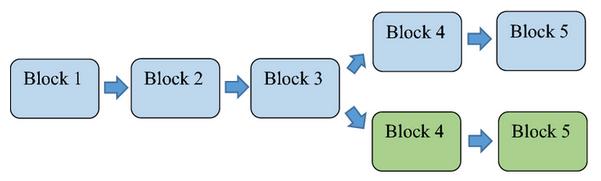
\includegraphics[scale=0.5]{./images/fork-01.png}
\captionof{figure}[https://www.researchgate.net/figure/The-fork-forms-and-disappears-in-the-PoW-Blockchain]{Ein Fork - die Blockchain ist nicht mehr einheitlich}
\end{center}

 Dies kann zwei Ursachen haben:
 \begin{enumerate}
 \item \textbf{Zufällig:} Wenn zwei Miner fast zeitgleich einen passend Hash für einen Block finden und diesen im Netzwerk verteilen. Aufgrund der endlichen Verteilungsgeschwindigkeit bekommen Full-Nodes unterschiedliche Blöcke, die sie aber erfolgreich verifizieren und an ihre lokale Blockchain anhängen.\\ Es gibt also gleich lange, aber unterschiedliche Chains im Netzwerk.\vspace{.4cm}\\
Diese Forks lösen sich aber meist innerhalb von wenigen (meist 5-6) weiteren Blöcken wieder auf - weil bis dahin wieder eine längste Chain existiert, von der man annimmt, dass sie die richtige Chain ist. Sie wird wieder auf alle Full-Nodes verteilt.
\begin{center}
%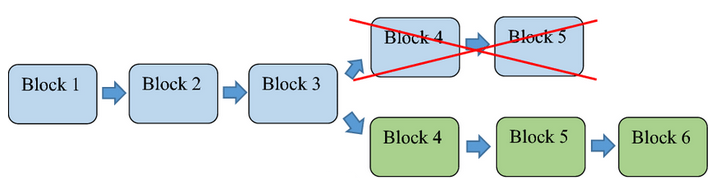
\includegraphics[scale=0.45]{./images/fork-02.png}
\captionof{figure}[https://www.researchgate.net/figure/The-fork-forms-and-disappears-in-the-PoW-Blockchain]{Ein Fork löst sich wieder auf - die Blockchain ist wieder einheitlich}
\end{center}

\item \textbf{Absichtlich:} Wenn es zu Regeländerungen im Sourecode kommt, z.B. wenn es Unstimmigkeit in der Community gibt. In diesem Fall spricht man von einem \textbf{Hard-Fork}. Ab diesem Zeitpunkt trennt sich das Netzwerk auf, manche Teilnehmer übernehmen die Regeländerung und manche nicht. Es entsteht dadurch eine neue Blockchain-Community wie z.B. beim Split von Ethereum und Ethereum-Classic im Juli 2016.
\end{enumerate}

\subsection{Mining} \label{mining}
Das Mining hat zwei wichtige Aufgaben. Zum einen die Verifizierung eines Blocks und zum anderen erzeugt es neue Coins.
\subsubsection{Verifizierung - Hashing}
Die Miner berechnen den Hash des aktuellen Blocks. Allerdings gibt der Bitcoin Algorithmus vor, dass der Hash mit einer bestimmten Anzahl von Nullen beginnen muss. Da der Hash nur geändert werden kann, wenn die Daten des Blocks geändert werden, wird dem Block ein weiteres Element hinzugefügt, das als \textbf{Nonce} bezeichnet wird.\\
Der Miner startet nun z.B: mit einer Nonce von 1 und berechnet die SHA256 Summe des Blocks. Wenn der resultierende Hash nicht die geforderte Anzahl von Anfangs-Nullen aufweist, erhöht er die Nonce auf 2 und berechnet wieder den Hash, usw. Es kann viele Billionen Berechnungen (Proof-of-work) brauchen, bis eine akzeptable Hashsumme gefunden wird.
\begin{center}
%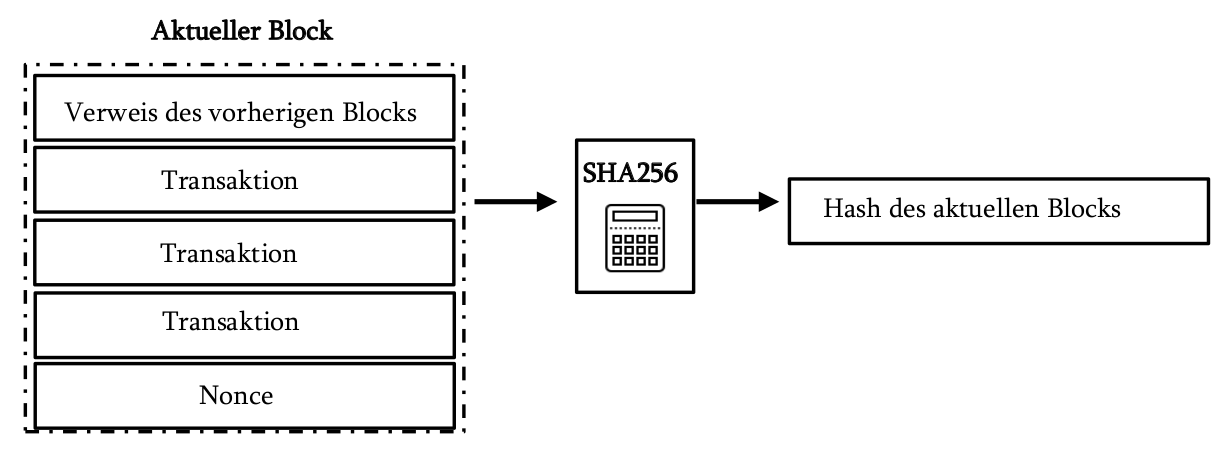
\includegraphics[scale=0.3]{./images/mining.png}
\captionof{figure}[Abbildung 24 aus dem Buch: Bitcoin ohne Vorkenntnisse]{Hashgenerierung aus den Daten eines Blocks inkl. der zusätzliche Variable \textbf{Nonce}}
\end{center}
Seit dem Bekanntwerden der Kryptowährungen gibt es Firmen die spezielle Mining (Hashing-) Geräte herstellen. Die wahrscheinlich bekannteste Firma ist \href{https://www.bitmain.com/}{\color{blue}www.bitmain.com}. Selbst kleine Geräte (Antminer) um wenige Tausend Dollar haben schon dreistellige \textbf{TH/s} (Terahashes pro Secunde) Werte.
\vspace{.3cm}\\
Wenn ein Miner nun den passenden Hash gefunden hat, schickt er den gelösten Block, inklusive seiner gefundenen \textbf{Nonce} an alle \textbf{Full-Nodes}. Diese kontrollieren, ob ein Hash mit der geforderten Anzahl an Nullen entsteht (eine einmalige SHA256 Berechnung). Ist das der Fall, wird der Block an die Blockchain angehängt und der Miner erhält seine \textbf{Belohnung}.
\subsubsection{Miner Belohnung und Transaction Fees}
Was ist die Motivation, das sehr rechen- und damit leider sehr energieintensive Mining durchzuführen? Warum macht das ein Miner, was hat er oder sie davon?\\
Es gibt zwei Verdienstmöglichkeiten:
\paragraph{Transaction Fees}
Im Bitcoin Netzwerk können nur ca. 3,3 Transaktionen pro Sekunde durchgeführt werden (Blocksize = 1 MByte -> ca. 2000 Transaktionen pro Block -> alle 10 Minuten ein neuer Block -> 2000/600 = 3,3). Wenn man nun eine dringende Transaktion machen möchte, kann man eine Transaktionsgebühr anbieten, damit die Miner die Transaktion in den aktuellen Block aufnehmen.\\
Ein Miner der einen Block löst (den richtigen Hash findet), bekommt alle Transaktionsgebühren der im Block enthaltenen Transaktionen.\\
Die anderen Miner gehen leer aus. Danach stürzen sich alle Miner sofort auf den nächsten Block und machen sich wieder auf die Suche nach der richtigen Nonce.\\
Die Transaktionsgebühren waren in der Vergangenheit starken Schwankungen unterworfen und lagen zeitweise über 60 USD pro Transaktion.
\begin{center}
%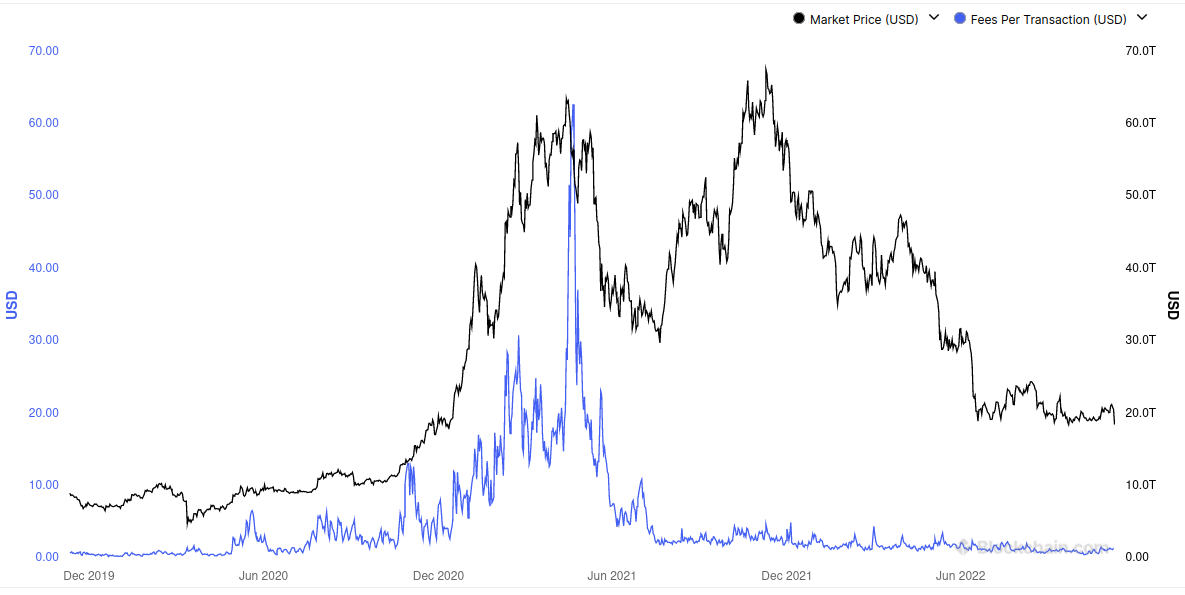
\includegraphics[scale=0.4]{./images/fees.png}
\captionof{figure}[https://www.blockchain.com/explorer/charts/fees-usd-per-transaction]{Transaktionsgebühren (Blau) und Bitcoin Marktwert (Schwarz)}
\end{center}
 
\paragraph{Belohnung - Block Subsidy}
Zusätzlich zu den Transaktionsgebühren
erhält der Miner, der den Block löst, eine Belohnung (neue Coins) die im Programm code verankert ist und je nach Kryptowährung unterschiedlich ist. Diese Belohnung nennt man Block Subsidy (Block-Subvention).\\
Bei Bitcoin war der Anfangswert der Block Subsidy 50 Bitcoins pro gefundenem Block. Da das Lösen eines Blocks im Mittel 10 Minuten dauert, wurden also alle 10 Minuten 50 neue Bitcoins in Umlauf gebracht.\\
Der Subsidy Wert halbiert sich allerdings alle 210 000 Blöcke (\textbf{Halving}), was einem Zeitraum von ca. 4 Jahren entspricht. Momentan (November 2022) gibt es \textit{"nur"} noch 6,25 Bitcoins pro gelöstem Block.
\begin{table}[h]
\centering
\begin{tabular}{|p{2cm}|p{2.5cm}|p{3.8cm}|p{3.7cm}|}
\hline 
\textbf{Zeitraum} &	\textbf{Block Subsidy} & \textbf{Neue Coins im Zeitraum} & \textbf{Alle Coins im Umlauf} \\
\hline 
2008-2012 & 50 & 10.500.000 BTC & 10.500.000 BTC\\
\hline
2012-2016 & 25 & 5.250.000 BTC & 15.750.000 BTC\\
\hline
2016-2020 & 12,5 & 2.625.000 BTC & 18.375.000 BTC\\
\hline
2020-2024 & 6,25 & 1.312.500 BTC & 19.687.500 BTC\\
\hline
2024-2028 & 3,125 & 656.250 BTC & 20.343.750 BTC\\
\hline
2028-2032 & 1.5625 & 328.125 BTC & 20.671.875 BTC\\
\hline 
. & . & . & .\\
\hline 
\end{tabular}
\caption{\textbf{Halving} - die Block Subsidy halbiert sich alle 4 Jahre}
\label{tabelle_1} 
\end{table}\\ 
Wie man aus Tabelle \ref{tabelle_1} auf Seite \pageref{tabelle_1} erkennen kann, nimmt die Anzahl der neu ausgeschütteten Coins ab und wird sich einen Wert von 21 Millionen BTC 
annähern.

\section{Teil der Blockchain werden}
Welche Schritte sind nun notwendig um selbst Teil der Blockchain zu werden?
\subsection{Meine Adresse auf der Blockchain}
Eine \textbf{Adresse} auf der Blockchain ist vergleichbar mit einer Konto Nummer, mit dem Unterschied, dass die Adresse öffentlich und für jeden Teilnehmer einsehbar ist! Jeder Teilnehmer kann durch Rückschau auf vergangene Transaktionen berechnen welche Adresse wie viele Bitcoins enthält!\\
Man kann z.B. auf \href{https://www.blockchain.com/btc/address/}{\color{blue}https://www.blockchain.com/btc/address/} nachsehen wie der "Kontostand" von Satoshi Nakamotos erster Adresse (hat mehrere) zur Zeit (November 2022) aussieht:
\begin{center}
%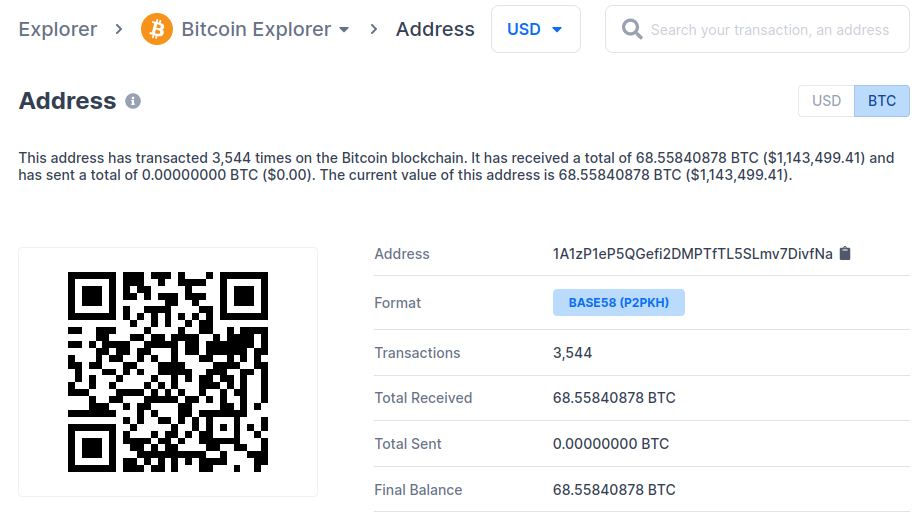
\includegraphics[scale=0.5]{./images/adress.png}
\captionof{figure}[https://www.blockchain.com/btc/address/1A1zP1eP5QGefi2DMPTfTL5SLmv7DivfNa]{"Kontostand" der Genesis Adresse - erste Adresse von Satoshi Nakamoto}
\end{center}
Die \textbf{Adresse} auf der Bitcoin Blockchain ist in Wirklichkeit der leicht abgewandelte \textbf{öffentliche Schlüssel (public key)} eines asymmetrischen Schlüsselpaares. Siehe Kapitel \ref{asym} auf Seite \pageref{asym} zur Erinnerung wie Puplic Key Encryption funktioniert.\\
Der public key wird aus einem zufällig gewählten private key (bei Bitcoin 256 Bit Länge) generiert.   
Aus diesem wird dann (mittels Hashfunktionen - zuerst SHA256 und dann RIPEMD160) die öffentliche Adresse (160 Bit = 20 Byte Länge) erstellt.
\subsection{Wallets}
Wallets sind kleine Programme die bei der Key-Erstellung und Verwaltung (eine Wallet kann mehrere Keys für mehreren Crypto-Währungen verwalten) helfen.
\begin{center}
\fcolorbox{green}{gruenlich}{\begin{minipage}{15cm}{
ACHTUNG: Die Wallets sind nicht Vergleichbar mit einer Geldtasche oder einem Konto, weil sie selber keine Coins verwalten, sondern nur die Adressen! Die Blockchain selbst ist mit ihren transparenten Transaktionen das "Konto".
}\end{minipage}}
\end{center}
\subsubsection{Arten von Wallets}
\paragraph{Hot Wallet}
Von einer Hot Wallet spricht man, wenn die Wallet online bei einer Handelsplattform (Exchange) liegt. Zum Beispiel bei \href{https://www.bitpanda.com}{\color{blue}www.bitpanda.com}.\\
Dies ist zwar bequem (Online Zugriff via Browser) aber sehr unsicher, da schon einige Exchanges gehackt worden sind oder zahlungsunfähig wurden oder der Betreiber alle Keys gestohlen hat und sich auf die Bahamas abgesetzt hat :(
\paragraph{Cold Wallet}
Die Wallet ist offline. Man unterscheidet noch zwischen:
\begin{itemize}
\item \textbf{Software Wallet} z.B. auf dem privaten PC Zuhause oder auf einem verschlüsselten USB-Stick. Ist sicher, aber Achtung wenn z.B. der USB Stick verloren geht oder der PC versehentlich entsorgt wird - siehe \href{https://futurezone.at/digital-life/festplatte-7500-bitcoin-muellhalde-finden-james-howells/402088129}{\color{blue}James Howell}, der im Jahr 2013 eine Festplatte mit Keys zu ca. 7500 BTC auf den Müll geworfen hat ;-)
\item \textbf{Hardware Wallets} sind spezielle Hardware und Software zur Key-Sicherung. Sie z.B. Firma \href{https://www.ledger.com/}{\color{blue}www.ledger.com}
\item \textbf{Paper Wallet} die Keys werden mit open source Software einmalig erzeugt und nur analog (z.B: auf einem Blatt Papier) gespeichert. Sehr sicher gegen online Angriffe aber sorgfältige Verwahrung ist ein Muss! 
\end{itemize}
\subsubsection{Key Erstellung}
Wie schon erwähnt hilft die Wallet bei der Key-Erstellung.\\
Als erstes wird der \textbf{private Key} (256 Bit) erstellt, entweder durch einen halb automatischen Algorithmus mit User Interaktion (z.B: Mouse Bewegungen) oder durch einen Zufallszahlengenerator. \\
Aus diesem wird mit Hilfe einer \textbf{elliptischen Kurven-Funktion} (siehe Kapitel \ref{ECC} auf Seite \pageref{ECC}) der zugehörige (unkomprimierte) \textbf{public Key} generiert.\\
Aus diesem wird dann (mittels Hashfunktionen - zuerst SHA256 und dann RIPEMD160) die öffentliche Adresse (160 Bit = 20 Byte Länge) erstellt.
\begin{center}
%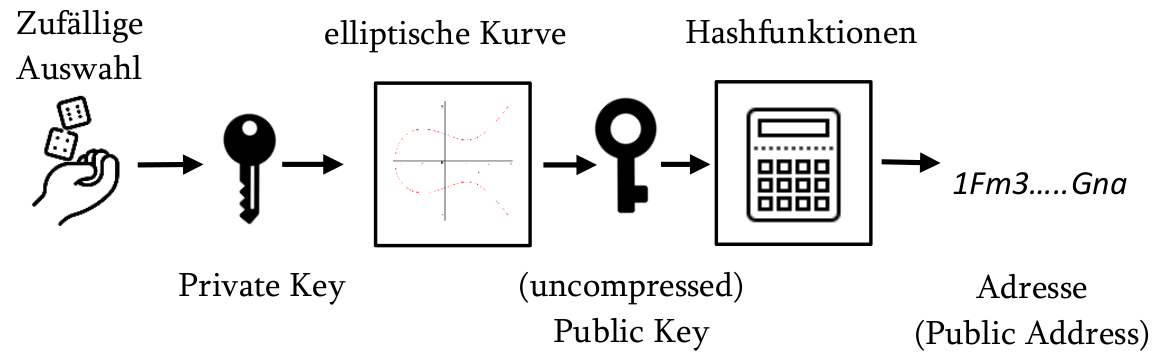
\includegraphics[scale=0.4]{./images/key_generation.png}
\captionof{figure}[Abbildung 17 aus dem Buch: Bitcoin ohne Vorkenntnisse]{Generierung der Bitcoin-Adresse}
\end{center}

\subsubsection{Eine Transaktion senden}
Eine weitere Aufgabe die von den Wallets erledigt wird, ist das Senden von Transaktionen.\\
Nehmen wir an, Alice möchte Bob einen Bitcoin (1 BTC) senden.\\
Die gewünschte Transaktion lautet dann: Von der öffentlichen Bitcoin-Adresse von Alice soll ein Bitcoin an die öffentliche Adresse von Bob geschickt werden.\\
Damit sichergestellt wird, dass diese Transaktion wirklich von Alice ausgeht, \textbf{signiert} sie sie mit ihrem \textbf{Private Key}. Siehe dazu Kapitel \ref{asym} auf Seite \pageref{asym}.\\
Diese signierte Transaktion (plus eine Transaktionsgebühr - siehe Kaptiel \ref{mining} Mining auf Seite \pageref{mining}) wird von der Wallet an alle umliegenden Miner und Nodes gesendet, welche sie wiederum weitersenden, bis jeder im Netzwerk diese Transaktion sehen kann.\\
Die Nodes überprüfen, ob der Absender genug Coins im Besitz hat (History der Blockchain).\\
Wenn die Transaktionsgebühr hoch genug ist, wird die Transaktion in den nächsten Block mit aufgenommen und wenn er voll ist (es passen ca. 4200 Transaktionen in einen Block) wird mit dem Mining begonnen.
\begin{center}
%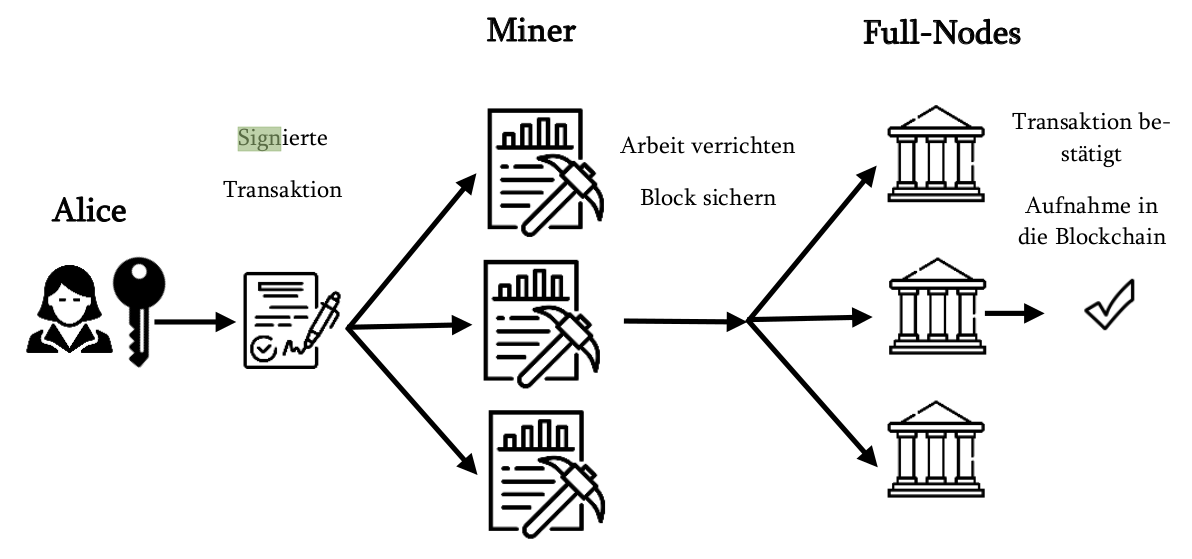
\includegraphics[scale=0.4]{./images/alice.png}
\captionof{figure}[Abbildung 20 aus dem Buch: Bitcoin ohne Vorkenntnisse]{Abfolge beim Senden einer Transaktion}
\end{center}

\section{Stablecoins - Coins zu Dollar}
Stablecoins werden verwendet um Crypto-Coins in eine reale Fiat-Währung wie den US-Dollar umzuwandeln.\\
Die Krypto-Tauschbörse \href{https://www.bitfinex.com/}{\color{blue}Bitfinex}
hat eine Kryptowährung erschaffen, die den Wert von einem US-Dollar abbildet.
Dafür wurden eine Milliarde US-Dollar auf einem Bankkonto hinterlegt und eine
Milliarde sogenannte \textbf{Tether} (USDT) zum Kauf angeboten.\\
Die Firma hinter Tether garantiert, dass wir für den Tether-Coin bei Bedarf auch einen US-Dollar ausbezahlt bekommen.\\
Bitfinex verdient nun, wie eine Bank, beim Tausch zwischen verschiedenen Coins und der Auszahlung (Rückkauf von Tether).\\
Kursschwankungen werden versucht auszugleichen:\\ 
Wenn die Coin-Nachfrage zu niedrig ist, gleicht Tether die Kursschwankungen
durch Kaufen des Coins aus. Ist die Coin-Nachfrage hingegen zu hoch, wirkt Te
ther dem entgegen, indem neue Coins ausgegeben werden, sodass der Nominalwert von 1 USD eingehalten werden kann.\vspace{.3cm}\\
Wichtig bei Stablecoins ist, wie auch im Papiergeldsystem, dass die Währung gedeckt ist. Gedeckt bedeutet, dass zu jedem Tether-Coin auch ein entsprechender US-Dollar auf einem Bankkonto eingefroren ist. Nur so kann der Wert von Tether sichergestellt werden. Stellen wir uns vor, es gäbe eine Milliarde Tether-Coins, aber es sind nur eine Million Dollar auf einem Bankkonto hinterlegt.\\
Aktuelles Beispiel (November 2022) wo dies gerade nicht mehr der Fall ist: \href{https://ftx.com/}{\color{blue}FTX}. Siehe \href{https://www.n-tv.de/wirtschaft/Bei-FTX-soll-mindestens-eine-Milliarde-Dollar-fehlen-article23713547.html}{\color{blue}FTX Zahlungsunfähigkeit}




\section{Probleme}
Bitcoin und die Crypto-Währungen werden häufig als das Zahlungsmittel der Zukunft verkauft. Es soll anonym, frei von Mittelsmännern (Banken) sein und keine Inflation aufweisen.\\
Anstelle einer stabilen Währung haben sie sich aber bis jetzt (November 2022) eher als hochspekulativ und instabil erwiesen.
\subsection{Hohe Volatilität}
Zu den grundlegenden hohen Kurschwankungen aufgrund des völlig unregulierten 24 Stunden Handels kommen noch Euphorie oder Panik hinzu. Zum Teil sind Tweets von Promis ausreichend, um massive Kursschwankungen auszulösen.
\subsubsection{Mittelsmänner}
Es braucht nach wie vor Mittelsmänner, statt Banken sind es nun \textbf{Crypto-Exchanges}. Auf Grund von fehlenden Regulierungen sind sie viel anfälliger gegen Missbrauch, gezielte Angriffe und Zahlungsausfall als traditionelle Banken.\\
Beispiel vom November 2022: \href{https://www.derstandard.at/story/2000140794202/kryptoboerse-kraken-will-mutmasslichen-ftx-hacker-identifiziert-haben}{\color{blue}FTX - Zahlungsausfall und Diebstahl}
\subsubsection{Fairness}
Auch von Fairness kann keine Rede sein, weil in beiden Konsensmechanismen (Proof-of-Work und Proof-of-Stake) immer die \textit{'starken'} oder \textit{'die schon viel besitzen'} belohnt werden.
\subsubsection{51\% Angriff} \label{51}
Bei Coins, die Proof-of-Work als Konsensmechanismus nutzen, kann eine Gruppe die über 51\% der gesamten Hashing-Power des Netzwerks besitzt, das Netzwerk komplett übernehmen. Sie sind schneller im Minen als alle anderen, und erzeugen so die längste Blockchain, welche von allen anderen Nodes als wahre Blockchain wahrgenommen wird.\\
Dies ist bei großen Coins wie Bitcoin zwar schwierig, aber nicht unmöglich. So erzielte der Mining-Pool GHash.IO im Juni 2014 über einen Zeitraum von 24 Stunden einen Anteil von etwa 55\% der Bitcoin-Hashrate.\\
Auf kleinere Coins werden aber immer wieder mit 51\% Angriffe durchgeführt. 
\subsubsection{Transaktionslimit}
ca. 3,3 Transaktionen pro Sekunde weil 1 MByte Blockgröße mit ca. 2000 Transaktionen und 10 min. Zeit für einen Block!\\
Führt im August 2017 zum Hard-Fork und der Abspaltung Bitcoin-Cash (hat nun 8 MB Blockgröße).\\
Zum Vergleich: Visa wickelt ca 65000 Transaktionen pro Sekunde ab, das sind fast 150 Millionen Transaktionen pro Tag!
\subsubsection{Finality}
Finality beschreibt, ab wann ein Teilnehmer der Blockchain sicher sein kann, dass seine Transaktion auch Teil der Blockchain - und somit wahr - ist. Da es ja immer wieder zu Forks kommen kann und sich die längste Blockchain nach meist 5-6 Blöcken (jeweils 10 Minuten pro Block) durchsetzt. Kann ich als Teilnehmer erst nach 6x10 Minuten sicher sein, ob meine Transaktion auch Teil der Blockchain ist!
\subsubsection{Energieaufwand bei Proof-of-Work}
Der Cambridge \href{https://ccaf.io/cbeci/index}{\color{blue}Bitcoin Electricity Consumption Index} hat das Mining des Bitcoin auf seinen Energieverbrauch hin untersucht. Zur Zeit (November 2022) liegt der Energieverbrauch bei ca.100 Terawattstunden. Im Vergleich dazu verbraucht Österreich pro Jahr ca. 70 Terawattstunden Energie.





\end{document}

%%%%%%%%%%%%%%%%%%%%%%%%%%%%%%%%%%%%%%%%%%%%%%%%%%%%%%%%%%%%%%%%%%%%
%%% Vorlagen
%%%%%%%%%%%%%%%%%%%%%%%%%%%%%%%%%%%%%%%%%%%%%%%%%%%%%%%%%%%%%%%%%%%%
\begin{cverbatim}
\end{cverbatim}

\begin{pverbatim}
\end{pverbatim}

\begin{center}
\fcolorbox{red}{rotlich}{\begin{minipage}{5cm}{
\fcolorbox{green}{gruenlich}{\begin{minipage}{15cm}{

}\end{minipage}}
\end{center}

\begin{figure}[h!]
\begin{center}
\includegraphics[scale=0.4]{./images/leistung05.eps}
\end{center}
\end{figure}
\FloatBarrier
%%%%%%%%%%%%%%%%%%%%%%%%%%%%%%%%%%%%%%%%%%%%%%%%%%%%%%%%%%%%%%%%%%%%%
\section{A}
\subsection{B}
\subsubsection{C}
\paragraph{D}
%%%%%%%%%%%%%%%%%%%%%%%%%%%%%%%%%%%%%%%%%%%%%%%%%%%%%%%%%%%%%%%%%%%%%